%-*- coding: utf-8 -*-
\documentclass[french,11pt]{article}
\usepackage{babel}
\DecimalMathComma

\usepackage{graphicx}
\usepackage[hidelinks]{hyperref}

% Fonts
\usepackage[T1]{fontenc}
\usepackage{gentium-otf}

% SI units
\usepackage{siunitx}

% Table becomes Tableau
\usepackage{caption}
\captionsetup{labelfont=sc}
\def\frenchtablename{Tableau}

%%%% GEOMETRY AND SPACING %%%%%%%%%%%%%%%%%%%%%%%%%%%%%%%%%%%%%%%%%%%%%%%
\usepackage{subcaption}

% % List management
\usepackage{enumitem}

\usepackage{etex}
\usepackage[tmargin=2cm,bmargin=2cm,lmargin=2cm,footnotesep=1cm]{geometry}

\parskip=1ex\relax % space between paragraphs (incl. blank lines)
%%%%%%%%%%%%%%%%%%%%%%%%%%%%%%%%%%%%%%%%%%%%%%%%%%%%%%%%%%%%%%%%%%%%%%

\usepackage[dvipsnames]{xcolor}
\usepackage{listings}
\lstset{%
  frame=single,                    % adds a frame around the code
  tabsize=2,                       % sets default tabsize to 2 spaces
  columns=flexible,                % doesn't add spaces to make the line fit the whole column
  basicstyle=\ttfamily,             % use monospace
  keywordstyle=\color{MidnightBlue},
  commentstyle=\color{Gray},
  stringstyle=\color{BurntOrange},
  showstringspaces=false,
}

%%% SYMBOLS %%%%%%%%%%%%%%%%%%%%%%%%%%%%%%%%%%%%%%%%%%%%%%%%%%%%%%%%%%
% % Math symbols
\usepackage{amsmath}
\usepackage{amssymb}
\usepackage{bm}

% Math symbols
\newcommand{\Acal}{\mathcal{A}}
\newcommand{\Bcal}{\mathcal{B}}
\newcommand{\Ccal}{\mathcal{C}}
\newcommand{\Ecal}{\mathcal{E}}
\newcommand{\Gcal}{\mathcal{G}}
\newcommand{\Ical}{\mathcal{I}}
\newcommand{\Kcal}{\mathcal{K}}
\newcommand{\Lcal}{\mathcal{L}}
\newcommand{\Ncal}{\mathcal{N}}
\newcommand{\Pcal}{\mathcal{P}}
\newcommand{\Qcal}{\mathcal{Q}}
\newcommand{\Rcal}{\mathcal{R}}
\newcommand{\Scal}{\mathcal{S}}
\newcommand{\Tcal}{\mathcal{T}}

\newcommand{\DD}{\mathcal{D}}
\newcommand{\FF}{\mathcal{F}}
\newcommand{\HH}{\mathcal{H}}
\newcommand{\LL}{\mathcal{L}}
\newcommand{\MM}{\mathcal{M}}
\newcommand{\OO}{\mathcal{O}}
\newcommand{\TT}{\mathcal{T}}
\newcommand{\UU}{\mathcal{U}}
\newcommand{\XX}{\mathcal{X}}
\newcommand{\YY}{\mathcal{Y}}
\newcommand{\ZZ}{\mathcal{Z}}

\newcommand{\CC}{\mathbb{C}}
\newcommand{\EE}{\mathbb{E}}
\newcommand{\NN}{\mathbb{N}}
\newcommand{\PP}{\mathbb{P}}
\newcommand{\RR}{\mathbb{R}}
\newcommand{\RRnp}{\mathbb{R}^{n \times p}}
\newcommand{\RRnn}{\mathbb{R}^{n \times n}}
\newcommand{\RRpp}{\mathbb{R}^{p \times p}}
\newcommand{\VV}{\mathbb{V}}


% Vectors
\makeatletter
\newcommand{\avec}{\vec{a}\@ifnextchar{^}{\,}{}}
\newcommand{\bb}{\vec{b}\@ifnextchar{^}{\,}{}}
\newcommand{\cvec}{\vec{c}\@ifnextchar{^}{\,}{}}
\newcommand{\gvec}{\vec{g}\@ifnextchar{^}{\,}{}}
\newcommand{\hh}{\vec{h}\@ifnextchar{^}{\,}{}}
\newcommand{\mm}{\vec{m}\@ifnextchar{^}{\,}{}}
\newcommand{\oo}{\vec{o}\@ifnextchar{^}{\,}{}}
\newcommand{\pp}{\vec{p}\@ifnextchar{^}{\,}{}}
\newcommand{\rr}{\vec{r}\@ifnextchar{^}{\,}{}}
\newcommand{\tvec}{\vec{t}\@ifnextchar{^}{\,}{}}
\newcommand{\uu}{\vec{u}\@ifnextchar{^}{\,}{}}
\newcommand{\uprime}{\vec{u'}\@ifnextchar{^}{\,}{}}
\newcommand{\vv}{\vec{v}\@ifnextchar{^}{\,}{}}
\newcommand{\vprime}{\vec{v'}\@ifnextchar{^}{\,}{}}
\newcommand{\ww}{\vec{w}\@ifnextchar{^}{\,}{}}
\newcommand{\xx}{\vec{x}\@ifnextchar{^}{\,}{}}
\newcommand{\yy}{\vec{y}\@ifnextchar{^}{\,}{}}
\newcommand{\zz}{\vec{z}\@ifnextchar{^}{\,}{}}
\newcommand{\aalpha}{\vec{\alpha}\@ifnextchar{^}{\,}{}}
\newcommand{\bbeta}{\vec{\beta}\@ifnextchar{^}{\,}{}}
\newcommand{\ttheta}{\vec{\theta}\@ifnextchar{^}{\,}{}}
\newcommand{\mmu}{\vec{\mu}\@ifnextchar{^}{\,}{}}
\newcommand{\xxi}{\vec{\xi}\@ifnextchar{^}{\,}{}}
\makeatother

% Hats
\newcommand{\thetahat}{{\widehat \theta}}
\newcommand{\hatn}{{\widehat n}}
\newcommand{\hatp}{{\widehat p}}
\newcommand{\hatm}{{\widehat m}}
\newcommand{\hatmu}{{\widehat \mu}}
\newcommand{\hatsigma}{{\widehat \sigma}}

\newcommand{\hatmle}[1]{\widehat{#1}_{\text{MLE}}}
\newcommand{\hatmap}[1]{\widehat{#1}_{\text{MAP}}}
\newcommand{\hatbys}[1]{\widehat{#1}_{\text{Bayes}}}

\DeclareMathOperator*{\argmax}{arg\,max}
\DeclareMathOperator*{\argmin}{arg\,min}

\newcommand{\cvn}{\xrightarrow[n \rightarrow +\infty]{}}
\newcommand{\cvproba}{\stackrel{\PP}{\longrightarrow}}
\newcommand{\cvps}{\stackrel{\text{p.s.}}{\longrightarrow}}
\newcommand{\cvltwo}{\stackrel{\Lcal^2}{\longrightarrow}}
\newcommand{\cvloi}{\stackrel{\Lcal}{\longrightarrow}}

% Sets
\newcommand{\zo}{\lbrace 0, 1 \rbrace}
\newcommand{\mopo}{\lbrace -1, 1 \rbrace}

% \newcommand{\lzeronorm}[1]{\left|\left|#1\right|\right|_0}
% \newcommand{\lonenorm}[1]{\left|\left|#1\right|\right|_1}
% \newcommand{\ltwonorm}[1]{\left|\left|#1\right|\right|_2}
% \newcommand{\lzeronorm}[1]{\|#1\|_0}
% \newcommand{\lonenorm}[1]{\|#1\|_1}
% \newcommand{\ltwonorm}[1]{\|#1\|_2}
\usepackage{mathtools}
\DeclarePairedDelimiter{\abs}{\lvert}{\rvert}
\DeclarePairedDelimiter{\norm}{\lVert}{\rVert}
\DeclarePairedDelimiter{\bignorm}{\bigg\lVert}{\bigg\rVert}
\DeclarePairedDelimiter{\innerproduct}{\langle}{\rangle}

\DeclarePairedDelimiter{\lzeronorm}{\lVert}{\rVert_0}
\DeclarePairedDelimiter{\lonenorm}{\lVert}{\rVert_1}
\DeclarePairedDelimiter{\ltwonorm}{\lVert}{\rVert_2}
%%%%%%%%%%%%%%%%%%%%%%%%%%%%%%%%%%%%%%%%%%%%%%%%%%%%%%%%%%%%%%%%%%%%%%


\begin{document}

\begin{center}
\bf\large ECUE21.2: Science des données \hfill
PC 6 -- Modèles linéaires pour la classification
\end{center}

\noindent
\hfill 7 juillet 2025.

\noindent
\rule{\textwidth}{.4pt}

\medskip

\paragraph{Pour aller à l'essentiel}
\begin{itemize}
\item Quelques questions sont assez techniques (calculs, optimisation). Le
  choix vous est donné d'admettre les résultats ou de les démontrer. Pendant la
  PC, il vaut mieux les admettre afin de pouvoir vous concentrer sur
  les aspects directement liés au cours de science des données.
\item Le but de cette PC est d'illustrer les principes de minimisation du risque empirique, maximisation de la vraisemblance, et régularisation avec deux algorithmes de classification : la \textbf{régression logistique} et les \textbf{machines à vecteurs de support} (ou \textbf{SVM}). Ces deux méthodes sont implémentées dans \texttt{scikit-learn}.
\end{itemize}

\section{Régression logistique}
Nous considérons ici un problème de classification binaire en
dimension $p$ : nous disposons d'un jeu d'apprentissage
$\DD = \{(\xx^i,~y^i)\}_{i=1, \dots, n}$ composé de $n$ individus étiquetés
$(\xx^i,~y^i) \in \RR^{p+1} \times \{0, 1\}.$

Nous considérons ici $\xx \in \RR^{p+1}$, après avoir ajouté un 1 à gauche d'un
vecteur $p$-dimensionnel, afin de simplifier les notations vectorielles et
matricielles comme dans la section 7.6.2 du poly :
$\beta_0 + \sum_{j=1}^p \beta_j x_j$ peut alors être noté
$\innerproduct{\bbeta,~\xx}.$ 

On appelle \textbf{fonction logistique} (à ne pas confondre avec la
\textit{fonction de coût logistique} de la section 7.4.2 du poly) la fonction
\begin{align*}
  \sigma: \RR & \rightarrow [0, 1]\\
  u & \mapsto \frac{1}{1+e^{-u}}. 
\end{align*}
Son graphe est représenté sur la figure~\ref{fig:logistic}. Cette fonction est
dérivable et sa dérivée vérifie (vous pouvez le vérifier)
\begin{equation}
  \sigma^\prime(u) = \sigma(u) (1-\sigma(u)) \text{ en tout point } u \in \RR.
  \label{eq:sigma_prime}
\end{equation}

\begin{figure}[h]
  \centering
  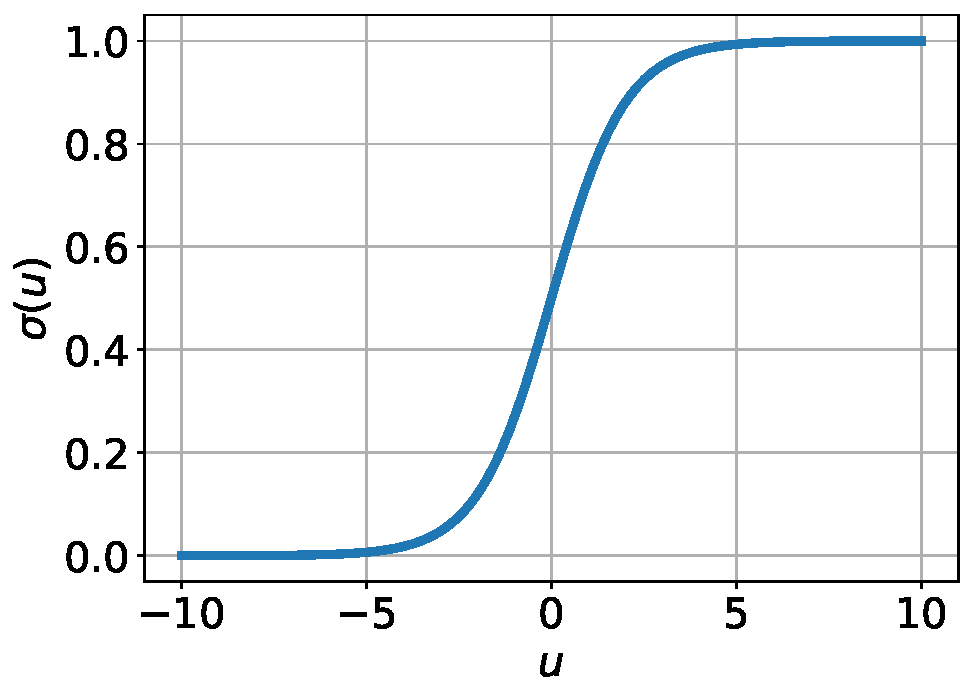
\includegraphics[width=0.5\textwidth]{figures/logistic}
  \caption{Graphe de la fonction logistique}
  \label{fig:logistic}
\end{figure}

\subsection{Minimisation du risque empirique}    
\begin{enumerate}
\item Pourquoi un modèle paramétrique linéaire, c'est-à-dire de la forme
  $f: \xx \mapsto \innerproduct{\bbeta,~\xx}$, n'est-il pas approprié pour un problème de
  classification binaire ?
\end{enumerate}

On pourrait utiliser un modèle linéaire comme \textit{fonction de décision} :
$f(\xx) \geq 0$ conduit à prédire une étiquette positive, et $f(\xx) < 0$
conduit à prédire une étiquette négative.

Dans le cas de la \textbf{régression logistique}, on préfère utiliser comme
fonction de décision la composition d'une fonction linéaire et de la fonction
logistique :
\begin{equation}
  f(\xx) = \sigma(\innerproduct{\bbeta,~\xx}).
  \label{eq:logistic_model}
\end{equation}
\begin{enumerate}[resume]
\item 
  Comment peut-on alors interpréter $f(\xx)$ ? Prêtez attention à l'espace
  d'arrivée de $\sigma$.
\item Utiliser cet espace des hypothèses et l'entropie croisée
  (définie à la section 7.4.2 du poly) comme fonction de coût pour poser l'apprentissage d'un
  classifieur binaire sous la forme de la minimisation d'un risque empirique.
\item Montrer ou admettre que le risque empirique est convexe. Admet-il un minimum global ? 
\item Comment minimiser le risque empirique ? On pourra montrer ou admettre que le gradient du risque empirique en $\bbeta$ vaut 
    \begin{equation*}
      \nabla_{\bbeta}R_n = - \frac1n \sum_{i=1}^n \left(y^i - \frac1{1 + e^{-\innerproduct{\bbeta,~\xx^i}}} \right) \xx^i.
    \end{equation*}
    Pour le calculer, on pourra poser
    $\sigma_i = \sigma(\innerproduct{\bbeta,~\xx^i})$ et commencer par exprimer
    $\nabla_{\bbeta} \sigma_i$ en fonction de $\xx^i$ et $\sigma_i$.
\end{enumerate}



\subsection{Formulation probabiliste}  
Nous considérons maintenant que notre jeu d'apprentissage est la réalisation de
l'échantillon aléatoire
$\left((X_1, Y_1), (X_2, Y_2), \dots, (X_n, Y_n) \right), $ constitué de $n$
copies i.i.d. de $(X, Y)$. Ici $X$ est un vecteur aléatoire à valeurs dans
$\RR^{p+1}$ et $Y$ une variable aléatoire discrète à valeurs dans $\{0,
1\}$. $\bbeta \in \RR^{p+1}$ est maintenant un paramètre à
estimer.

% \paragraph{Vraisemblance} Nous avons jusqu'à présent défini la vraisemblance uniquement pour une variable
% aléatoire à densité ou pour une variable aléatoire discrète (voir
% \texttt{erratum\_estimation.pdf}). Cette définition peut être étendue à un
% vecteur aléatoire réel $Z$ dont certaines composantes, notées $U$, sont à
% densité et les autres, notées $V$, sont discrètes, de la façon suivante. On
% note $g$ la densité du vecteur aléatoire à densité $U$. Une réalisation $\zz$
% de $Z$ peut être décomposée comme $(\uu,~\vv)$, avec $\uu$ la composante à densité et $\vv$ la composante discrète. Alors la vraisemblance d'un
% échantillon $((\uu^1, \vv^1), (\uu^1, \vv^2), \dots, (\uu^n, \vv^n))$ de $Z$
% est définie par
%   \begin{equation}
%     \label{eq:likelihood}
%     L(\zz^1, \zz^2, \dots, \zz^n; \theta) = \prod_{i=1}^n \PP(V = \vv^i|U=\uu^i) g(\uu^i),
%   \end{equation}
%   où $g$ et $\PP_{V|U=\uu}$ peuvent toutes deux être paramétrées par $\theta$. 

\paragraph{Vraisemblance} Nous avons défini (Section 3.6 du poly) la
vraisemblance dans le cadre de l'estimation ponctuelle. Ici, nous allons nous
intéresser, comme dans le contexte des régressions paramétriques (sections
7.5.3 et 7.5.4), à l'estimation du \textit{vecteur} $\bbeta \in \RR^{p+1}$, à
partir d'un échantillon d'un \textit{vecteur aléatoire} $Z$ dont certaines
composantes, notées $U$, sont à densité et les autres, notées $V$, sont
discrètes. Pour calculer la vraisemblance d'un échantillon de $Z$ paramétré par
$\bbeta$, il faut pouvoir exprimer la loi de $Z$ sous la forme
$\PP_Z = f_{\bbeta} \mu,$ avec $\mu$ une mesure et $f_{\bbeta}$
$\mu$-mesurable. On y arrive en exprimant $\PP_{Z;\bbeta} = \PP_{V|U} \PP_U$ et
en exprimant $\PP_{V|U}$ grâce à la fonction de masse de $V|U$ et $\PP_U$ grâce
à la densité de $U$.


\begin{enumerate}
\item 
  Posons $g_X$ la densité de $X$. Écrire la log-vraisemblance du jeu
  d'apprentissage $\DD$ en fonction de $\PP(Y=1 | X=\xx^i)$.
\item Dans cette log-vraisemblance, remplacer $\PP(Y=1 | X=\xx^i)$ par sa
  valeur telle que modélisée dans la section~1.1. Qu'en conclure sur
  l'estimateur par maximum de vraisemblance ?
\end{enumerate}


\subsection{Régularisation}

\begin{enumerate}
\item Écrire la version régularisée $\ell_2$ de la minimisation du risque
  empirique proposée plus haut. % Commenter sur l'optimisation de ce problème :
  % a-t-on une solution unique ? Comment l'atteindre ?
  Quel est l'effet de ce
  régulariseur sur le modèle appris ?
\item Même question pour la régularisation $\ell_1$.
\end{enumerate}


\section{Machine à vecteurs de support}
Nous considérons ici toujours un problème de classification binaire en
dimension $p$, mais allons utiliser $\{-1, 1\}$ pour les étiquettes. Nous
disposons d'un jeu d'apprentissage $\DD = \{(\xx^i, y^i)\}_{i=1, \dots, n}$
composé de $n$ individus étiquetés
$(\xx^i, y^i) \in \RR^{p} \times \{-1, 1\}.$

% Nous considérons ici $\xx \in \RR^{p+1}$, après avoir ajouté un 1 à gauche d'un
% vecteur $p$-dimensionnel, afin de simplifier les notations vectorielles et
% matricielles comme dans la section 7.6.2 du poly :
% $\beta_0 + \sum_{j=1}^p \beta_j x_j$ peut alors être noté
% $\innerproduct{\bbeta,~\xx}.$ 

\subsection{SVM à marge rigide}
Nous supposons ici que les données sont linéairement séparables : il existe un
hyperplan de $\RR^p$ tel que tous les individus de la classe positive
(étiquetés $+1$) soient d'un côté de cet hyperplan et tous les individus de la
classe négative (étiquetés $-1$) de l'autre. Un tel exemple est illustré sur la figure~\ref{fig:linearly_separable}.

\begin{figure}[h]
  \begin{subfigure}[t]{0.45\textwidth}
    \centering
    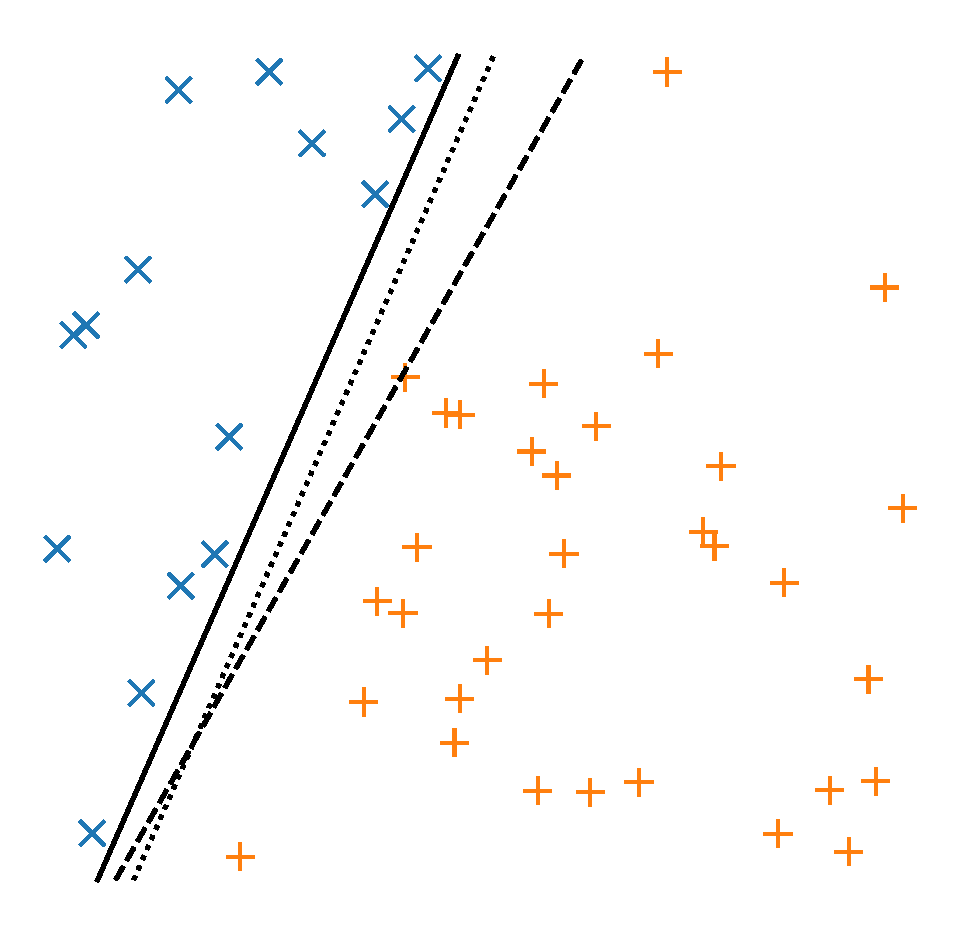
\includegraphics[width=\textwidth]{figures/linearly_separable}  
    \caption{Données linéairement séparables ($p=2$) et 3 exemples d'hyperplan
      séparateur.}
    \label{fig:linearly_separable}
  \end{subfigure} \hfill
  \begin{subfigure}[t]{0.45\textwidth}
    \centering
    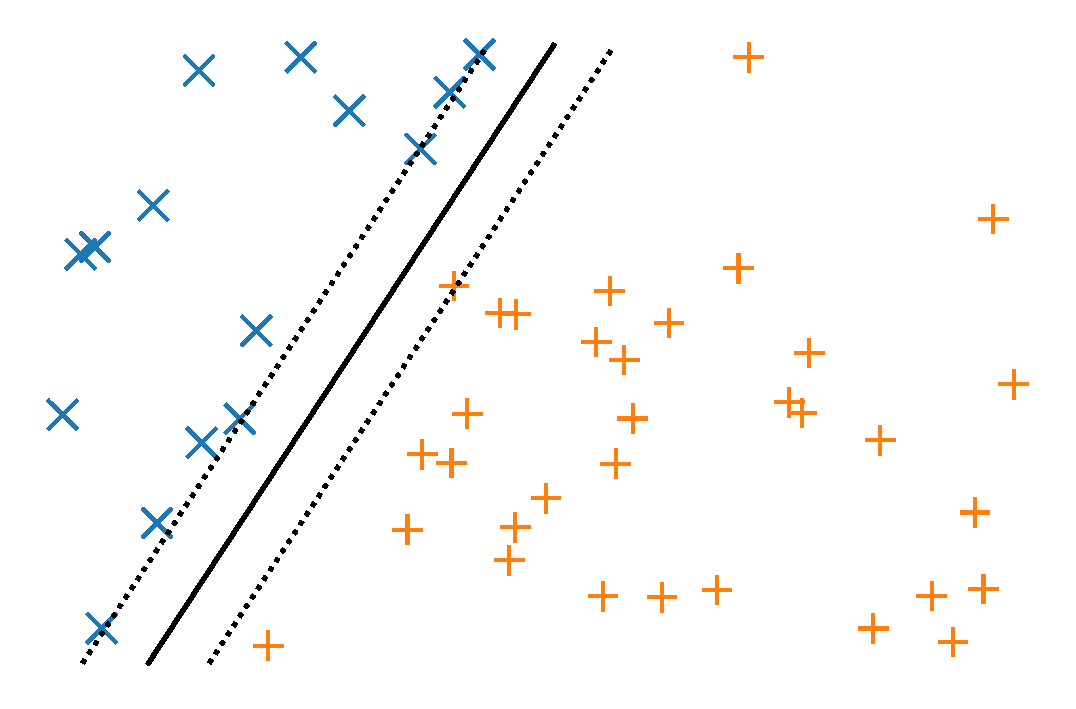
\includegraphics[width=\textwidth]{figures/margin}  
    \caption{Les droites en pointillés représentent les hyperplans parallèles à
      l'hyperplan séparateur, d'équations $\innerproduct{\ww,~\xx} + b = \pm 1$.}
    \label{fig:margin}
  \end{subfigure} 
\end{figure}


\begin{enumerate}
\item Si nous posons $\ww \in \RR^p$, $b \in \RR$ tels que
  $\innerproduct{\ww,~\xx} + b = 0$ soit l'équation d'un tel hyperplan, quel
  est le signe de $y^i \left(\innerproduct{\ww,~\xx^i} + b\right)$ pour $i=1, \dots, n$?
\item Cet hyperplan fait donc office de modèle de classification. Quelle est
  l'équation de la fonction de décision du modèle ? Quel est le modèle de classification
  binaire correspondant ?
\item Nous allons maintenant définir la \textbf{marge} d'un tel classifieur :
  c'est la distance entre l'hyperplan  $H$ d'équation $\innerproduct{\ww,~\xx} + b = 0$ et le
  point de $\DD$ qui en est le plus proche. Comparez les 3 hyperplans de la
  figure~\ref{fig:linearly_separable} : lequel a la plus petite marge ? La plus
  grande marge ?
\item Le principe des classifieurs à vaste marge (\textit{large margin
    classifiers} en anglais) est de choisir, parmi plusieurs classifieurs
  possibles, celui qui a la plus grande marge. Voyez-vous pourquoi ? 
\end{enumerate}

Nous allons maintenant chercher à déterminer $\ww \in \RR^p$ et $b \in \RR$
tels que l'hyperplan $H$ d'équation $\innerproduct{\ww,~\xx} + b = 0$ ait la plus
grande marge possible.

Pour cela, nous allons poser définir deux hyperplans parallèles à $H$ :
\begin{equation*}
  \begin{cases}
    H_- : \innerproduct{\ww,~\xx} + b = -1 & \\
    H_+ : \innerproduct{\ww,~\xx} + b = +1, & \\
  \end{cases}
\end{equation*}
de sorte à ce que le(s) point(s) positif(s) le(s) plus proche(s) de $H$ soit sur $H_+$ et que le(s) point(s) négatif(s) le(s) plus proche(s) de $H$ soit sur $H_-$.
Les valeurs $\pm 1$ sont choisies sans perte de généralité, utiliser une constante $c>0$ à la place de $1$ reviendrait à diviser $\ww$ et $b$ par $c$.
Ces hyperplans sont représentés en pointillés sur la figure~\ref{fig:margin}.


\begin{enumerate}[resume]
\item Cela signifie que $H_-$ et $H_+$ sont à la même distance de $H$. Pourquoi
  cela est-il compatible avec l'idée de chercher un hyperplan $H$ de marge
  maximale ? 
\item La zone entre $H_+$ et $H_-$ est parfois appelée « zone d'indécision ». Pourquoi ?
\item Les points situés \textit{sur}  $H_+$ et $H_-$ sont appelés \textbf{vecteurs de support} et donnent leur nom à cette méthode : \textbf{machine à vecteurs de support} en français, \textbf{support vector machine (SVM)} en anglais.

  Voyez-vous d'où vient leur nom ?  Pour comprendre, supposez que vous
  déplaciez un tel point d'une distance $\epsilon$ faible ; comment cela
  affecterait-il $H$, $H_+$ et $H_-$ ? Même question pour un point situé loin
  de $H_+$ (ou $H_-$).
\item Quelle est la valeur de la marge ?
\item Les observations $\xx^i$ étant situées à l'extérieur de la zone
  d'indécision, quelle est l'inégalité vérifiée par
  $y^i \left(\innerproduct{\ww,~\xx^i} + b \right)$ pour $i=1, \dots, n$ ?
\item Poser le problème d'optimisation sous contraintes correspondant à maximiser la marge tout en assurant que l'inégalité de la question précédente est vraie pour $i=1, \dots, n$.
Montrer qu'il est équivalent à 
\begin{equation}
  \label{eq:hard-margin-svm}
    \argmin_{\ww \in \RR^p, b \in \RR} \frac{1}{2} \ltwonorm{\ww}^2 \text{ ~t.q.~ } 
    y^i \left(\innerproduct{\ww, \xx^i} + b \right)\geq 1, i=1, \dots, n.
  \end{equation} 
\item Identifier la formulation~\eqref{eq:hard-margin-svm} avec la minimisation d'un risque empirique régularisé : quel est l'espace des hypothèses ? Quelle est la fonction de perte ? Quel est le régulariseur ?
\item Montrer (ou admettre) que cette formulation est équivalente à
  \begin{align*}
    \max_{\aalpha \in \RR^n} & 
                               \sum_{i=1}^n  \alpha_i- \frac{1}{2} \sum_{i=1}^n \sum_{l=1}^n \alpha_i \alpha_l y^i y^l \innerproduct{\xx^i,~\xx^l} \\
    \nonumber \text{ t. q. }  & \sum_{i=1}^n \alpha_i y^i = 0;\,\, \alpha_i \geq 0,
                                i=1, \dots, n,
  \end{align*}
  et que si on appelle $(\ww^*, b^*)$ un minimiseur du problème d'optimisation
  posé à la question précedente, et $\alpha^*$ un maximiseur du problème
  ci-dessus, alors :

  \begin{equation*}
    \begin{cases}
  \ww^* = \sum_{i=1}^n \alpha_i^* y^i \xx^i & \\
  \alpha_i^* \left(y^i \left(\innerproduct{\ww^*,~\xx^i} + b^*\right) - 1 \right) = 0 & \text{ pour tout } i=1, \dots, n.\\
\end{cases}
\end{equation*}
\item Que dire de la valeur de $\alpha_i^*$ pour un vecteur de support, par opposition à un autre point du jeu d'entraînement ? On partira de
  \begin{equation*}
    \alpha_i^* \left(y^i \left(\innerproduct{\ww^*,~\xx^i} + b^*\right) - 1 \right) = 0  \text{ pour tout } i=1, \dots, n.
  \end{equation*}
  \end{enumerate}



\subsection{Pour aller plus loin : SVM à marge souple}
Dans le cas non-séparable, on utilise la fonction de perte dite \textit{hinge},
définie par
\begin{align*}
  L_{\text{hinge}} : \{-1, 1\} \times \RR & \rightarrow \RR \\
  y, f(\xx) & \mapsto
              \begin{cases}
                0 & \mbox{ si } y f(\xx) \geq 1 \\
                1 - y f(\xx) & \mbox{ sinon.}
              \end{cases}
\end{align*}
De manière plus compacte, la perte hinge peut aussi s'écrire 
\begin{equation*}
  \label{eq:hinge-loss}
  L_{\text{hinge}}(f(\xx), y) = \max\left(0, 1 - y f(\xx) \right) = \left[ 1 - y f(\xx)\right]_+. 
\end{equation*}

La perte hinge est positive quand un point est situé du mauvais côté non pas de
l'hyperplan séparateur $H$, mais de $H_+$ pour un point d'étiquette positive
(respectivement, de $H_-$ pour un point d'étiquette négative).

La SVM à marge souple est la solution du problème d'optimisation
\begin{equation}
  \argmin_{\ww \in \RR^p, b \in \RR} \frac{1}{2} \ltwonorm{\ww}^2 + 
  C \sum_{i=1}^n \left[ 1 - y^i  \left(\innerproduct{\ww,~\xx^i} + b\right) \right]_+.
  \label{eq:soft-margin-svm}
\end{equation}

\begin{enumerate}
\item Identifier la formulation~\eqref{eq:soft-margin-svm} avec la minimisation
  d'un risque empirique régularisé.
\item En introduisant une variable d'ajustement (ou variable d'écart ; on
  parle de {\it slack variable} en anglais) 
  $\xi_i = \left[ 1 - y^i f(\xx^i)\right]_+$ pour chaque observation du jeu
  d'entraînement, le problème d'optimisation~\ref{eq:soft-margin-svm} est
  équivalent à
  \begin{align}
    \label{eq:soft-margin-svm-2}
    \argmin_{\ww \in \RR^p, b \in \RR, \xxi \in \RR^n} & \frac{1}{2} \ltwonorm{\ww}^2 + 
                                                         C \sum_{i=1}^n \xi_i  \\
    \nonumber \text{ t. q. }   &
                                 \begin{cases}
                                   y^i \left(\innerproduct{\ww,~\xx^i} + 
                                     b\right) \geq 1 - \xi_i, & \\
                                   \xi_i \geq 0 & \text{ pour tout } i=1, \dots, n
                                 \end{cases}\\
  \end{align}
  Montrer en suivant la même démarche que pour la question 12 de la section précédente que le problème~\eqref{eq:soft-margin-svm-2} est équivalent à :
  \begin{align}
    \label{eq:soft-margin-dual-pb}
    \max_{\aalpha \in \RR} & 
                             \sum_{i=1}^n  \alpha_i- 
                             \frac{1}{2} \sum_{i=1}^n \sum_{l=1}^n \alpha_i \alpha_l y^i y^l \innerproduct{\xx^i,~\xx^l} \\
    \nonumber \text{ t. q. } & \sum_{i=1}^n \alpha_i y^i = 0 \text{ et }  0 \leq \alpha_i
                               \leq C, \text{ pour tout } i=1, \dots, n.
  \end{align}
  
  et que si on appelle $(\ww^*, b^*)$ un minimiseur du
  problème~\eqref{eq:soft-margin-svm-2}, et $\alpha^*$ un maximiseur du
  problème ci-dessus, alors :
  \begin{equation*}
    \begin{cases}
      \ww^* = \sum_{i=1}^n \alpha_i^* y^i \xx^i & \\
      \alpha_i^* \left(y^i \left(\innerproduct{\ww^*,~\xx^i} + b^*\right) - 1 \right) = 0 & \\
      % \alpha^*_i \left(\innerproduct{\ww^*,~\xx^i} + b^*\right) = 0 & \\
      (C-\alpha^*_i) \left[ 1 - y^i \left( \langle \ww, \xx^i \rangle + b
      \right)\right]_+ = 0 & \text{ pour tout } i=1, \dots, n.
    \end{cases}
  \end{equation*}
\item Que dire maintenant de la valeur de $\alpha_i^*$ pour un vecteur de support, par opposition à un autre point du jeu d'entraînement ? On partira de 
  \begin{equation*}
    \begin{cases}
      \alpha_i^* \left(y^i \left(\innerproduct{\ww^*,~\xx^i} + b^*\right) - 1 \right) = 0 & \\
      % \alpha^*_i \left(\innerproduct{\ww^*,~\xx^i} + b^*\right) = 0 & \\
      (C-\alpha^*_i) \left[ 1 - y^i \left( \langle \ww, \xx^i \rangle + b
      \right)\right]_+ = 0 & \text{ pour tout } i=1, \dots, n.
    \end{cases}
  \end{equation*}
\end{enumerate}
\end{document}

%%% Local Variables:
%%% mode: latex
%%% TeX-master: t
%%% End:
